\section{Analisi}
\label{sec:analisi}
In questa sezione verrà effettuata un'analisi sui risultati mediati su 30 simulazioni,
comparando il modello base con il modello esteso e infine con un modello allo stato dell'arte.

\subsection{Modello Base}
Nelle figure \ref{fig:analisi-base-evacuated} e \ref{fig:analisi-base-casualties} vengono mostrate le percentuali di evacuati
e di morti nel tempo al variare del numero di auto e pedoni.
%
Come si può notare dalla figura \ref{fig:analisi-base-evacuated}, il numero di pedoni non influenza la percentuale di pedoni evacuati nel tempo.
%
Per quanto riguarda le auto, più è alto il numero di auto più tempo è richiesto per evacuare e inoltre più bassa è la percentuale di auto evacuate alla fine della simulazione.
%
Osservando la percentuale di evacuati totali si può notare che un numero minore di auto permette di evacuare il numero maggiore di agenti.
I casi con probabilità di pedoni del 75\% e 100\% si ottiene la stessa percentuale massima di agenti evacuati,
tuttavia il caso con probabilità 75\% ha un andamento più veloce per la presenza delle auto.

\begin{figure}[ht]
    \centering
    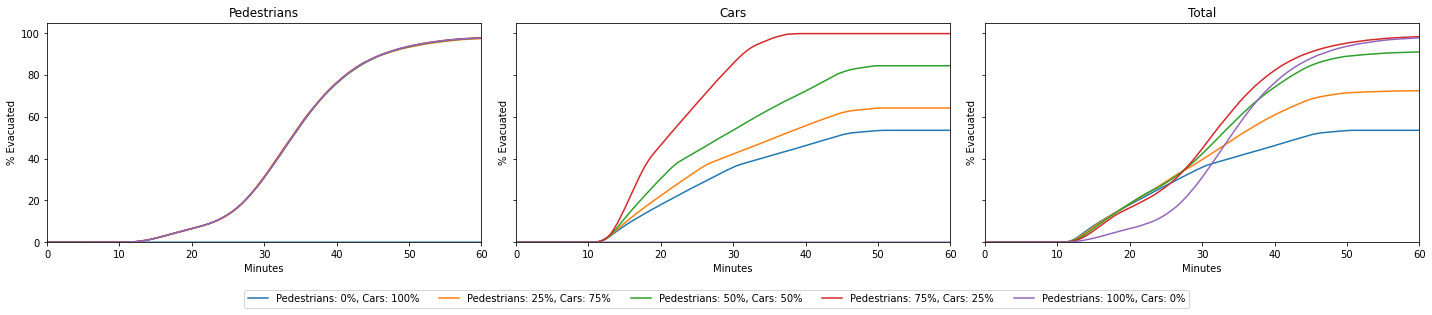
\includegraphics[width=\textwidth]{images/analisi/base-evacuated.png}
    \caption{Percentuale degli evacuati nel tempo al variare del numero di agenti con il modello base.}
    \label{fig:analisi-base-evacuated}
\end{figure}

Per quanto riguarda le percentuali di mortalità (Fig. \ref{fig:analisi-base-casualties}), possono essere fatte analisi simili a quelle in precendenza
per il numero di evacuati.
Per i pedoni in tutti i casi la percentuale di vittime rimane sotto al 2\%, mentre osservando le auto e le vittime totali
risulta una mortalità maggiore all'aumentare del numero di auto fino a un massimo di circa 50\%.
I casi con meno vittime sono con una probabilità di auto del 25\% e il caso solo pedoni che hanno risultati molto simili.

\begin{figure}[ht]
    \centering
    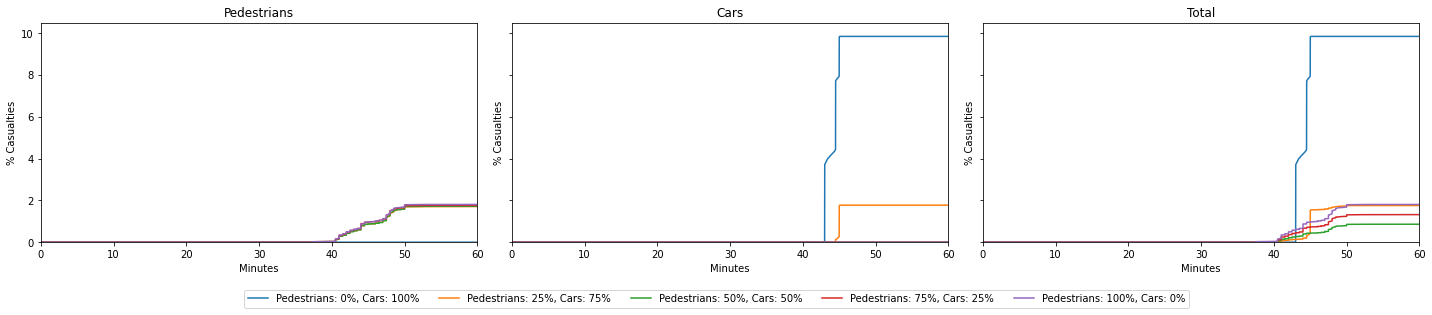
\includegraphics[width=\textwidth]{images/analisi/base-casualties.png}
    \caption{
        Percentuale delle vittime nel tempo al variare del numero di agenti con il modello base.
        %
    }
    \label{fig:analisi-base-casualties}
\end{figure}

Nella figura \ref{fig:analisi-base-evtimes} vengono riportate le percentuali di agenti evacuati nel tempo e il tempo in cui evacuano in media.
%
Nel caso con solo pedoni si ha un enorme picco vicino a 32 minuti con un tempo medio di 34 minuti e all'aumentare del numero di auto
il tempo medio di evacuzione si abbassa fino a 26 minuti nel caso con solo auto.

Nel caso con probabilità di auto del 25\% sembra formarsi un secondo picco più basso nei primi minuti probabilmente dovuto alle auto, mentre il secondo ai pedoni.
Questi picchi tendono ad appiattirsi con l'aumentare del numero di auto.

Inoltre si può notare come con un numero maggiore di auto considerate minore è la percentuale di agenti che evacuano negli ultimi minuti.
Questo poichè, come già evidenziato nella figura \ref{fig:analisi-base-evacuated}, le auto evacuano più velocemente dei pedoni.

\begin{figure}
    \centering
    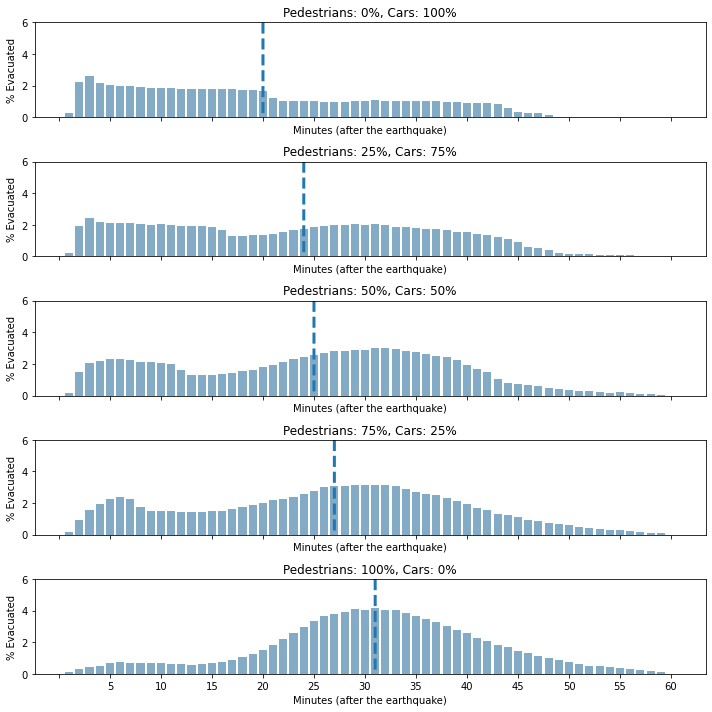
\includegraphics[width=\textwidth]{images/analisi/base-evtimes.png}
    \caption{
        Distribuzione del tempo di evacuzione in percentuale al variare del numero di agenti e tempo medio di evacuazione.
    }
    \label{fig:analisi-base-evtimes}
\end{figure}

\pagebreak

\subsection{Modello Esteso}
Nonostante l'introduzione della variazione della velocità per i pedoni,
la percentuale di pedoni evacuati risulta molto simile al variare del numero di pedoni (Fig. \ref{fig:analisi-new-evacuated}).
Si può notare una piccola differenza tra il minuto 30 e il minuto 40 per il caso con solo pedoni.

Il caso con una percentuale di auto evacuate maggiore è quello con una probabilità di auto del 25\%.
Il caso con solo auto, al contrario di come si possa pensare, non è il caso peggiore e ha un numero di evacuati simile ai casi
con probabilità di auto di 75\% e 50\%.

In generale il numero di auto evacuate è molto più basso rispetto a quello dei pedoni.

Considerando i contributi di auto e pedoni, al diminuire del numero di auto considerate cresce il numero totale di evacuati alla fine della simulazione,
fino al caso migliore con solo pedoni.

\begin{figure}[ht]
    \centering
    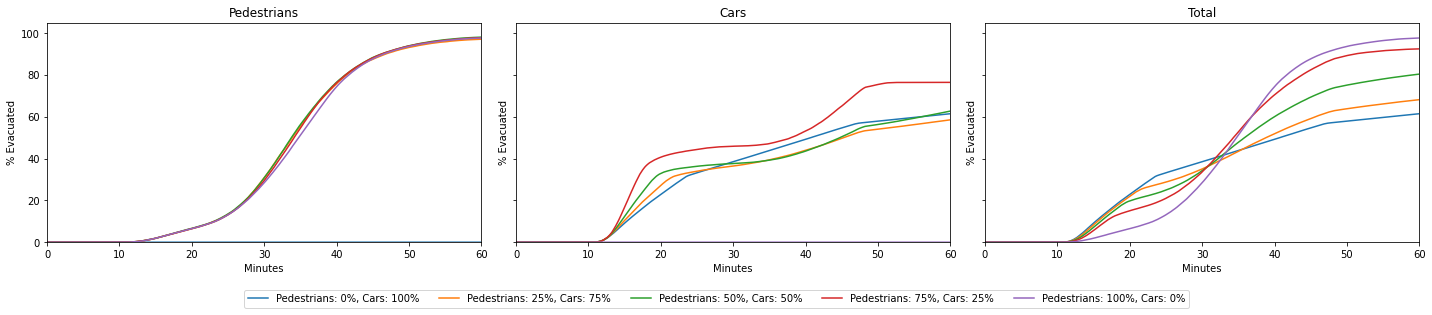
\includegraphics[width=\textwidth]{images/analisi/new-evacuated.png}
    \caption{Percentuale degli evacuati nel tempo al variare del numero di agenti con il modello esteso.}
    \label{fig:analisi-new-evacuated}
\end{figure}

Anche per le percentuali di morti (Fig. \ref{fig:analisi-new-casualties}) analisi simili alle percentuali di evacuati (Fig. \ref{fig:analisi-new-evacuated})
possono essere fatte.
%
Si può vedere come al variare del numero di pedoni considerati non ci siano differenze significative,
mentre per le auto la percentuale di vittime sale al crescere del numero di auto considerate.

In generale la percentuale di vittime per le auto è molto più alta rispetto a quella dei pedoni
con un massimo di poco più del 50\% nel caso con una probabilità di auto del 75\% che risulta con una mortalità superiore anche al caso solo auto.
%
Il numero di vittime totali cresce al crescere del numero di auto e il caso con solo auto è quello con la percentuale di mortalità maggiore.

\begin{figure}[ht]
    \centering
    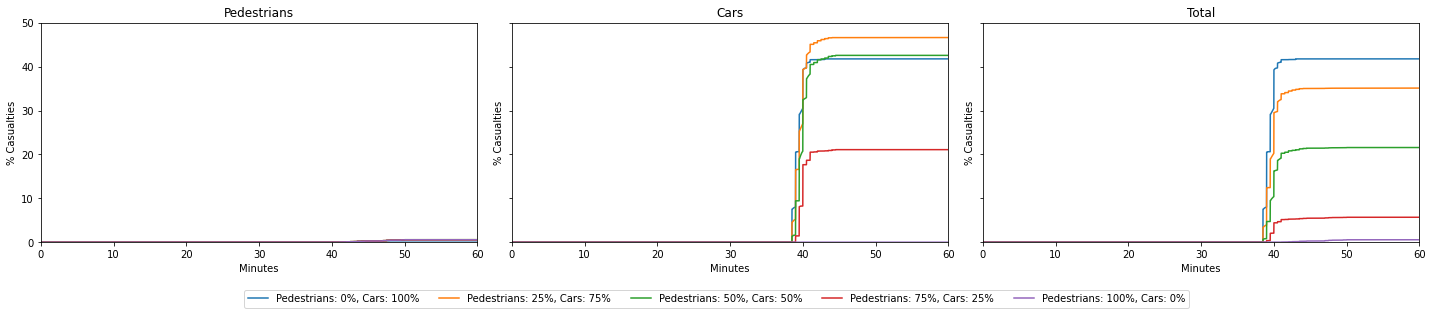
\includegraphics[width=\textwidth]{images/analisi/new-casualties.png}
    \caption{Percentuale delle vittime nel tempo al variare del numero di agenti con il modello esteso.}
    \label{fig:analisi-new-casualties}
\end{figure}

\pagebreak

Nella figura \ref{fig:analisi-new-evtimes} vengono riportate le percentuali di agenti evacuati nel tempo
e il tempo in cui evacuano in media.
%
In modo analogo al modello base il tempo medio di evacuazione si abbassa e sembrano formarsi due picchi nel caso con una probabilità di auto del 25\% per poi appiattirsi
all'aumentare del numero di auto.


\begin{figure}
    \centering
    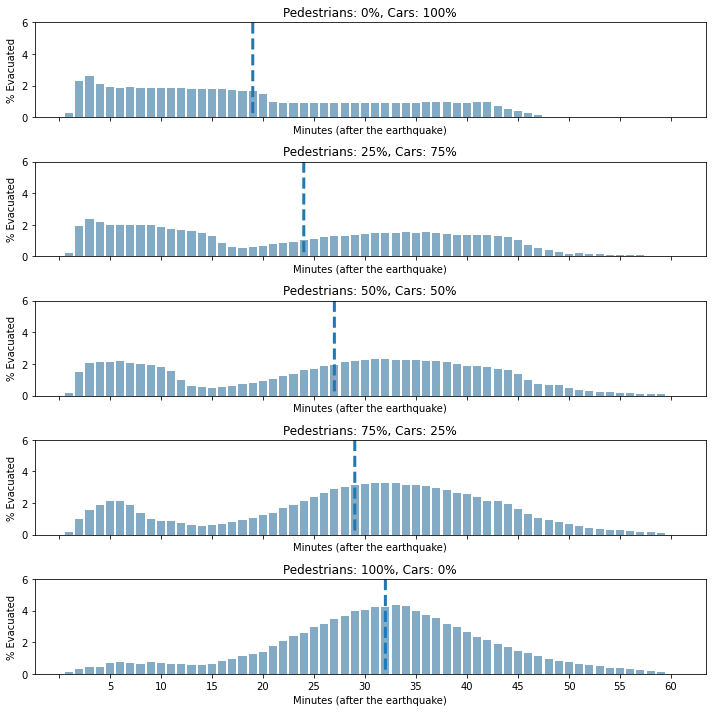
\includegraphics[width=\textwidth]{images/analisi/new-evtimes.png}
    \caption{Distribuzione del tempo di evacuzione in percentuale al variare del numero di agenti e tempo medio di evacuazione.}
    \label{fig:analisi-new-evtimes}
\end{figure}

\pagebreak

\subsection{Comparazione Modello Base e Modello Esteso}
In questa sottosezione verrano comparati il modello base e il modello esteso analizzando
le percentuali di evacuati e di vittime per poi passare a comparazioni spaziali,
in particolare mostrando l'effetto della gestione delle intersezioni durante la simulazione.

\subsubsection*{Percentuale di Evacuati e di Vittime}

\begin{figure}[ht]
    \centering
    \begin{subfigure}{0.45\textwidth}
        \centering
        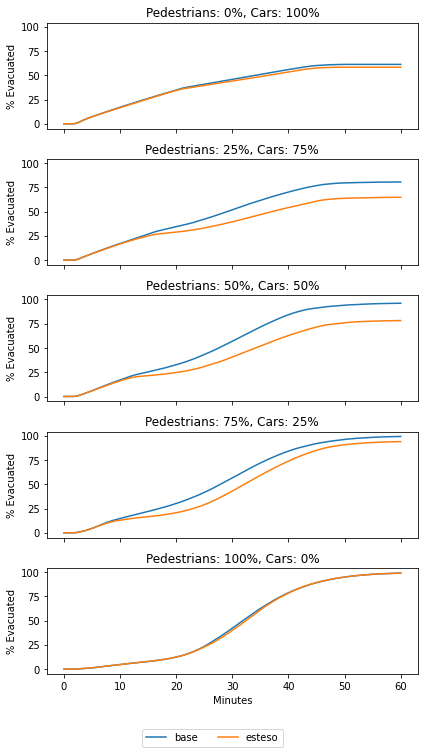
\includegraphics[width=\textwidth]{images/analisi/comparison-total-evacuated.png}
    \end{subfigure}
    \hfill
    \begin{subfigure}{0.45\textwidth}
        \centering
        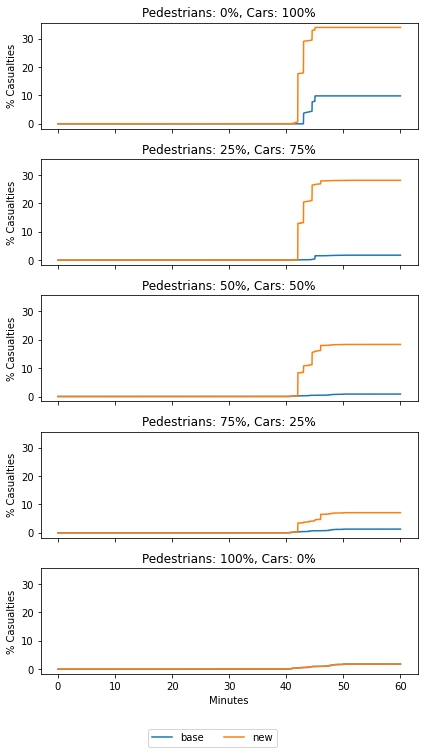
\includegraphics[width=\textwidth]{images/analisi/comparison-total-casualties.png}
    \end{subfigure}
    \caption{Comparazione tra modello base e modello esteso delle percentuali di evacuati (sinistra) e di vittime (destra) al variare del numero di agenti.}
    \label{fig:analisi-comparison-total-ec}
\end{figure}

Osservando la figura \ref{fig:analisi-comparison-total-ec} è possibile comparare le percentuali di evacuati e di vittime nel tempo al variare del numero di agenti tra i due modelli.
In generale il modello esteso presenta un numero minore di evacuati e un numero maggiore di vittime rispetto al modello base.
Questo può essere sintomo dell'effetto delle intersezioni che creando rallentamenti causano una mortalità maggiore,
infatti la percentuale di evacuati del modello esteso presenta un andamento più lento rispetto al modello di partenza.
Per entrambi i modelli la percentuale di evacuati decresce e la percentuale di vittime cresce all'aumentare del numero di auto considerate.
Inoltre per entrambi i modelli le prime vittime si verificano dopo 40 min.
Gli unici casi in cui il modello esteso e quello base hanno risultati molto simili sono il caso con solo pedoni e il caso solo auto,
ovvero i casi in cui l'effetto delle intersezioni è minimo.

\pagebreak

\subsubsection*{Percentuale di Evacuati nel Tempo}

Come già detto in precedenza le distribuzioni della percentuale di evacuati nel tempo del modello base e del modello esteso
presentano un andamento simile (Fig. \ref{fig:analisi-comparison-evtimes}). Il tempo medio di evacuazione abbastanza simile per i due modelli,
leggermente più alto per il modello esteso con una probabilità di pedoni di 75\%.

\begin{figure}[ht]
    \centering
    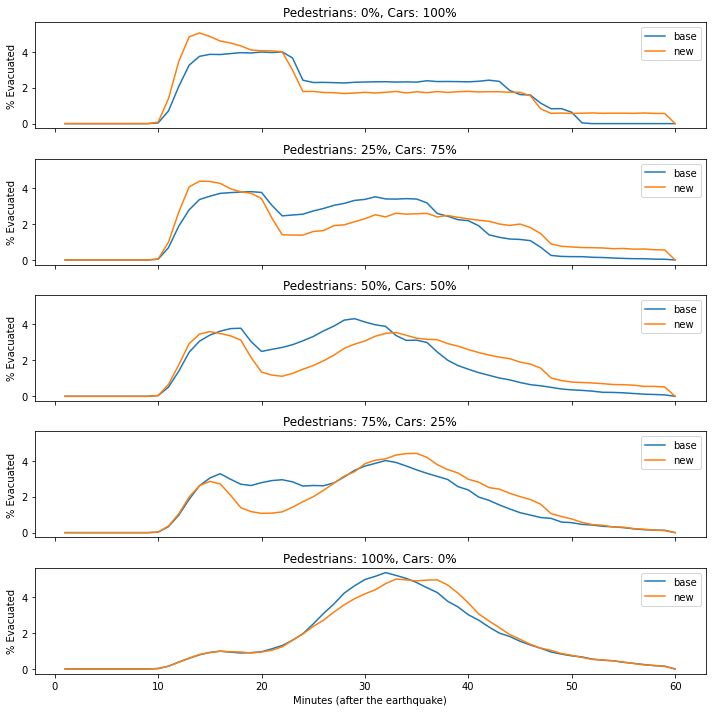
\includegraphics[width=0.9\textwidth]{images/analisi/comparison-evtimes.png}
    \caption{Comparazione delle distribuzioni dei tempi di evacuazione al variare del numero di agenti.}
    \label{fig:analisi-comparison-evtimes}
\end{figure}

\pagebreak

\subsubsection*{Tempo Impiegato per Evacuare}
Un'ulteriore comparazione riguarda il tempo che impiegano auto e pedoni per evacuare.
Come mostrato nella figura \ref{fig:analisi-comparison-evtimes2} per quanto riguarda le auto, il modello base presenta un andamento descresente per il tempo medio richiesto per evacuare al diminuire del numero di auto considerate.
Le auto impiegano in media tempi maggiori con il modello esteso rispetto a quello base.
%
I pedoni invece non presentano alcun cambiamento significativo al variare del numero di agenti e del modello considerato.

Per entrambi i modelli un pedone impiega in media un tempo di 19 minuti per evacuare e un massimo di 34 minuti.
Per le auto invece il tempo medio di evacuazione per il modello base è 11 minuti e per il modello esteso 14 minuti,
con tempi massimi rispettivamente di 38 e 41 minuti.

\begin{figure}[ht]
    \centering
    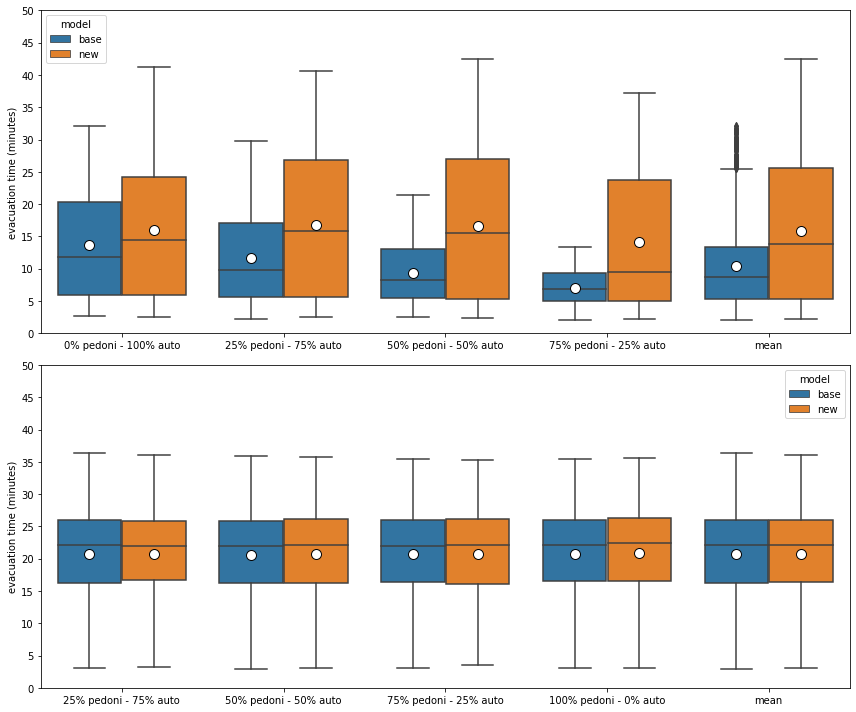
\includegraphics[width=\textwidth]{images/analisi/comparison-evtimes2.png}
    \caption{
        Comparazione dei tempi di evacuazione al variare del numero di agenti e nel caso medio distinti per auto (sopra) e pedoni (sotto).
    }
    \label{fig:analisi-comparison-evtimes2}
\end{figure}

\pagebreak

La figura \ref{fig:analisi-comparison-ev-times-map} mostra i tempi di evacuazione mediati tra gli agenti che partono dallo stesso nodo della rete,
mediati a loro volta tra tutte le configurazioni di auto e pedoni.

In generale gli agenti che partono dalla costa impiegano più tempo rispetto agli altri che sono più vicini ai rifugi.

Confrontando i pedoni al variare del modello usato non si riscontrano cambiamenti significativi nei tempi di evacuazione.
Mentre nel caso delle auto si nota che il modello esteso introduca dei rallentamenti rispetto al modello base, soprattuto lungo la costa.

\begin{figure}[ht]
    \centering
    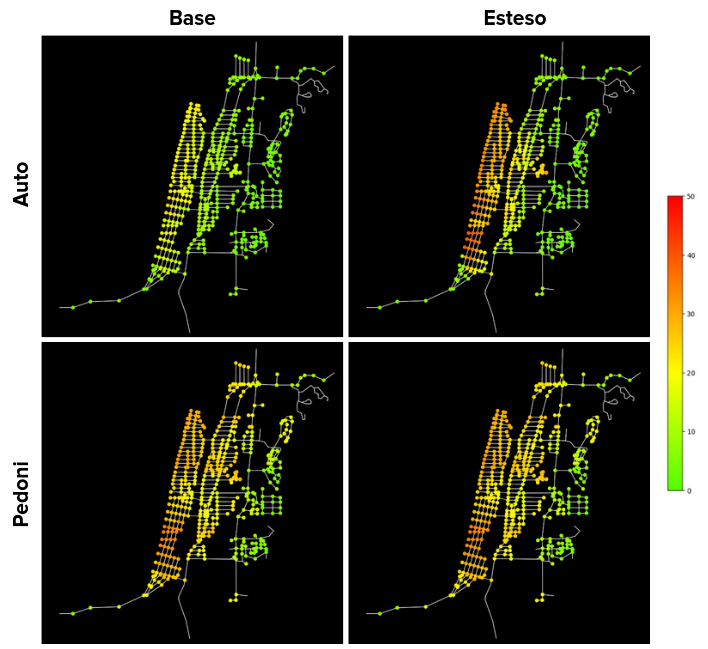
\includegraphics[width=\textwidth]{images/analisi/comparison-evtimes-map.png}
    \caption{Comparazione dei tempi di evacuazione mediati tra gli agenti che partono dallo stesso nodo della rete. }
    \label{fig:analisi-comparison-ev-times-map}
\end{figure}

\pagebreak


% \subsubsection*{Strade Critiche}
% Un'ulteriore analisi per valutare l'effetto dell'estensione del modello è quella di evidenziare in quali strade si verificano 
% più vittime al variare del numero di auto e pedoni. 
% %
% Nella figura \ref{fig:analisi-comparison-critical-links1} viene mostrato come si distribuisce la percentuale di mortalità nelle strade 
% al variare del numero di auto e pedoni e riportata la percentuale media. 

% Il modello base (Fig. \ref{fig:base-link-casualties}) nei casi con un numero di auto minore o uguale al 50\%
% non presenta differenze significative e si hanno tante strade con una percentuale bassa di vittime, 
% mentre negli altri due casi ci sono poche strade con una percentuale alta.

% Il modello esteso (Fig. \ref{fig:new-link-casualties}) invece presenta una strada comune per tutti casi 
% in cui sono presenti delle auto che contribuisce a più del 50\% delle vittime.
% %
% In generale in tutti i casi la maggior parte delle strade con più vittime sono diverse tra i due modelli a eccezione del caso 
% 100\% pedoni.
% %
% Le strade segnate come critiche corrispondono a quelle con una percentuale media maggiore del 5\% e sono mostrate nella figura \ref{fig:analisi-comparison-critical-links2}.

% \begin{figure}[ht]
%     \centering
%     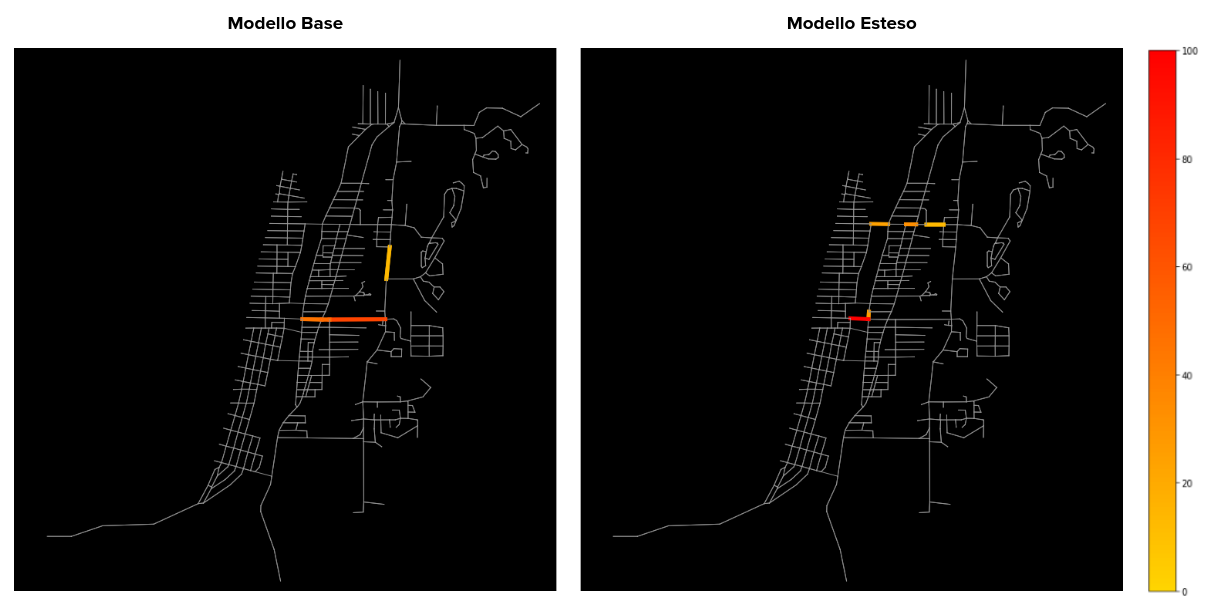
\includegraphics[width=0.8\textwidth]{images/analisi/casualties-map.png}
%     \caption{strade critiche trovate per i due modelli.}
%     \label{fig:analisi-comparison-critical-links2}
% \end{figure}

% \newpage

% \begin{figure}[ht]
%     \centering
%     \begin{subfigure}{0.475\textwidth}
%         \centering
%         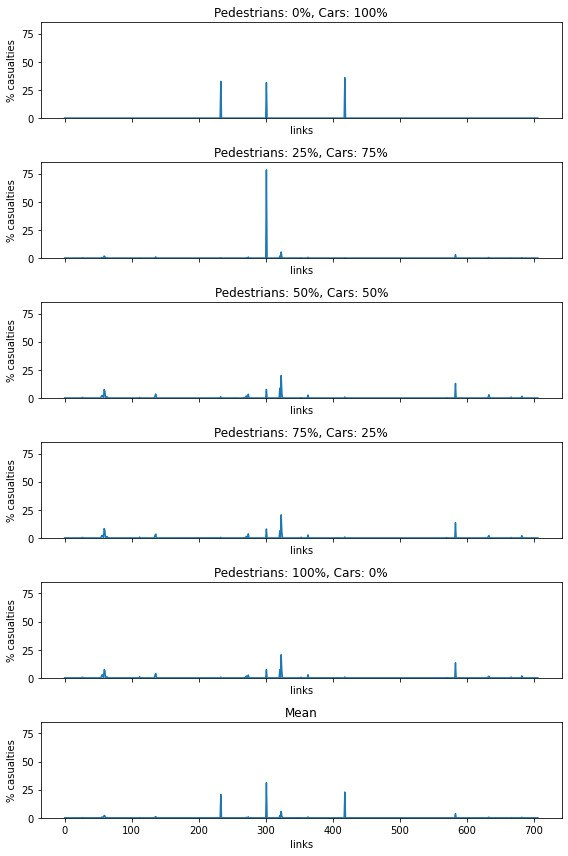
\includegraphics[width=\textwidth]{images/analisi/base_links_casualties}
%         \caption{Modello base}
%         \label{fig:base-link-casualties}
%     \end{subfigure}
%     \hfill
%     \begin{subfigure}{0.475\textwidth}
%         \centering
%         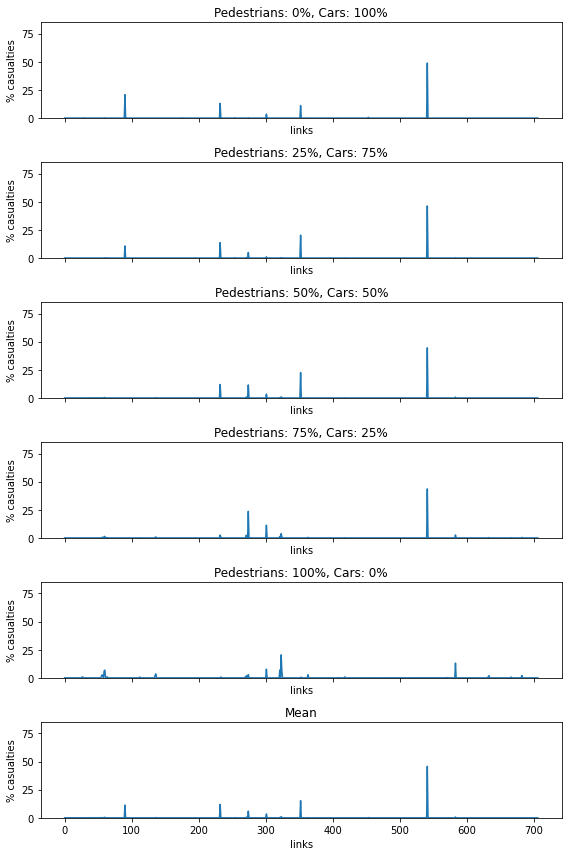
\includegraphics[width=\textwidth]{images/analisi/new_links_casualties}
%         \caption{Modello esteso}
%         \label{fig:new-link-casualties}
%     \end{subfigure}
%     \caption{Comparazione delle percentuali di mortalità nelle strade al variare del numero di auto e pedoni.}
%     \label{fig:analisi-comparison-critical-links1}
% \end{figure}


\newpage

\subsection{Analisi Intersezioni}
In questa sottosezione verranno descritte le analisi effettuate sulle intersezioni per valutare l'effetto dell'estesione
del modello. Per ogni intersezione sono stati analizzati la percentuale di vittime e il flusso in entrata e in uscita, comparando
i due modelli. Inoltre solo per il modello esteso sono stati analizzati anche i tempi medi di attesa nelle intersezioni,
poichè nel modello base non c'è attesa.

\subsubsection*{Percentuale di Vittime}
Nella figura \ref{fig:analisi-comparison-critical-ints1} vengono mostrate le percentuali di mortalità nelle intersezioni gestite per i due modelli al variare del numero di
agenti e il caso mediato. Inoltre le intersezioni sono ordinate per distanza crescente dal mare.

La percentuale di vittime in un'intersezione è il numero di vittime su ogni strada in entrata nell'intersezione sul numero di vittime totale.

In generale le intersezioni hanno una percentuale di mortalità non superiore al 10\%.
Nei casi con solo pedoni e solo auto i risultati sono molto simili.


\begin{figure}[ht]
    \centering
    \begin{subfigure}{0.475\textwidth}
        \centering
        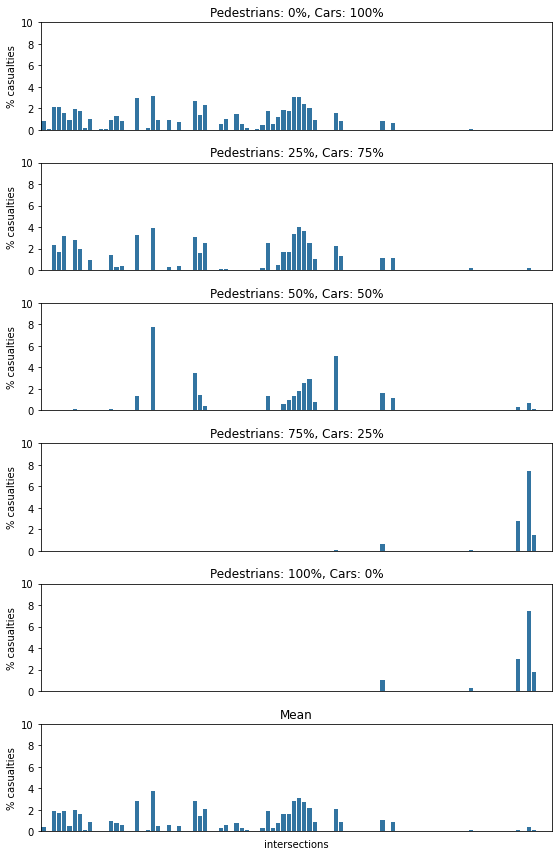
\includegraphics[width=\textwidth]{images/analisi/comparison-critical-ints-base.png}
        \caption{Modello base}
        \label{fig:base-ints-casualties}
    \end{subfigure}
    \hfill
    \begin{subfigure}{0.475\textwidth}
        \centering
        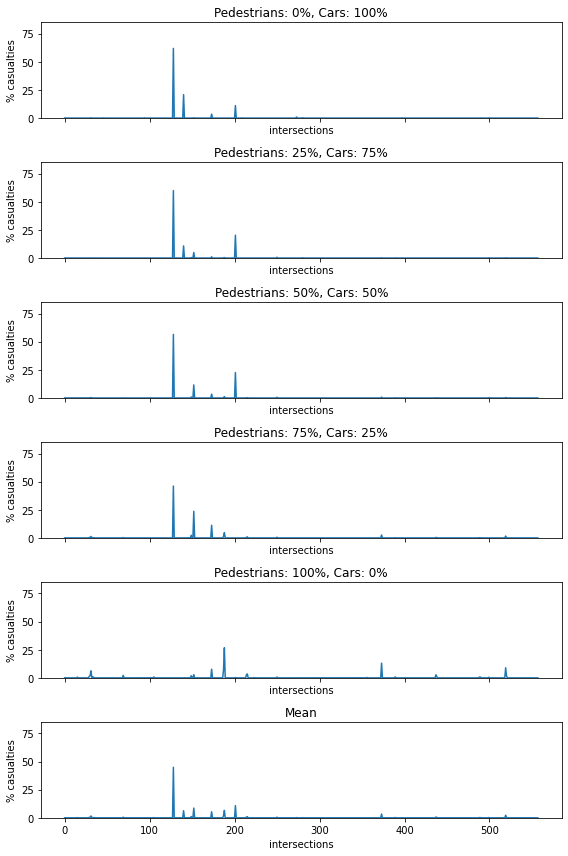
\includegraphics[width=\textwidth]{images/analisi/comparison-critical-ints-new.png}
        \caption{Modello esteso}
        \label{fig:new-ints-casualties}
    \end{subfigure}
    \caption{%
        Comparazione delle percentuali di mortalità nelle intersezioni al variare del numero di auto e pedoni.
        Le intersezioni sono ordinate per distanza crescente dal mare.
    }
    \label{fig:analisi-comparison-critical-ints1}
\end{figure}

Per quanto riguarda il caso con probabilità di auto del 75\%, entrambi i modelli condividono valori relativamente alti di mortalità per molte intersezioni,
ma nel modello esteso risultano leggermente più bassi.

Nei casi con probabilità di auto del 50\% e del 25\% il modello esteso ha una percentuale di mortalità distribuita su più intersezioni.

Come si può notare dall'ordine delle intersezioni (Fig. \ref{fig:analisi-comparison-critical-ints1}), i casi con più pedoni
hanno più vittime nelle intersezioni più distanti, mentre i casi con più auto hanno più vittime nelle intersezioni più vicine al mare per
via delle code che si formano in caso di congenstione.

In media le percentuali di mortalità per i due modelli risultato simili come si può vedere anche nella figura \ref{fig:analisi-comparison-critical-ints2}.


\begin{figure}[ht]
    \centering
    \begin{subfigure}{0.475\textwidth}
        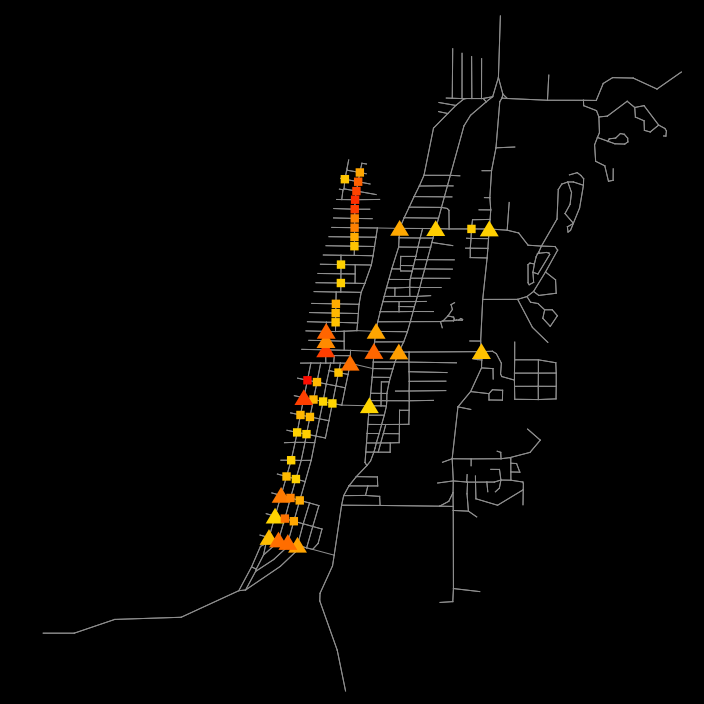
\includegraphics[width=\textwidth]{images/analisi/base_critical_ints_map.png}
        \caption{Modello base}
    \end{subfigure}
    \hfill
    \begin{subfigure}{0.475\textwidth}
        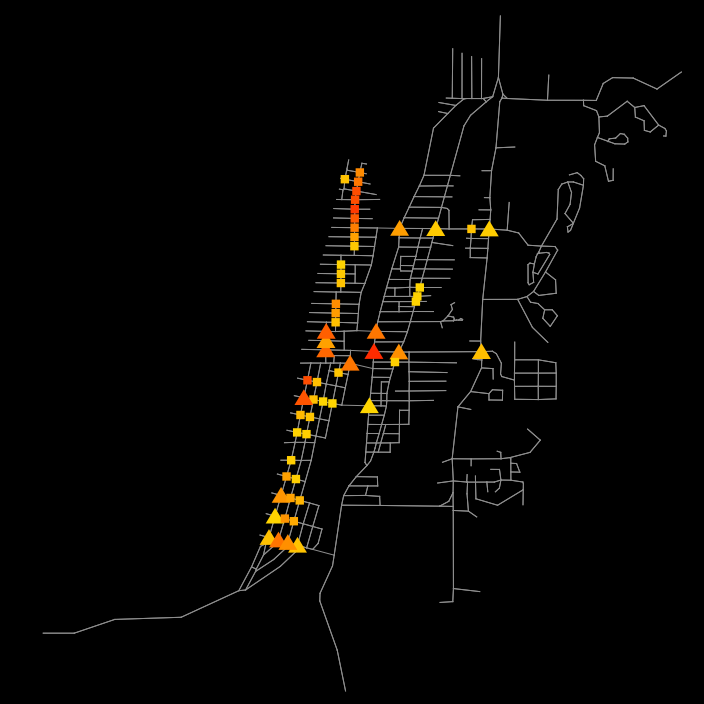
\includegraphics[width=\textwidth]{images/analisi/new_critical_ints_map.png}
        \caption{Modello esteso}
    \end{subfigure}
    \caption{Percentuali di vittime medie per ogni intersezione distinte per tipo: TWSC (quadrati), AWSC (triangoli).}
    \label{fig:analisi-comparison-critical-ints2}
\end{figure}

Nella figura \ref{fig:analisi-comparison-critical-ints2} vengono mostrate le percentuali di vittime nella rete
distinte in base al tipo di intersezione: TWSC, AWSC.

% TODO: commenti su TWSC, AWSC...

\subsubsection*{Flusso}
Per ogni intersezione è stato calcolato il flusso in entrata e in uscita sommando i valori di ogni strada al variare del numero di auto e pedoni.

Come si nota nella figura \ref{fig:analisi-comparison-in-out-flow-ped},
il flusso dei pedoni non presenta particolari differenze tra modello base ed esteso, nonostante le modifiche apportate ai pedoni.

Per entrambi i modelli il flusso in entrata e in uscita in ogni intersezione è molto simile.
Inoltre all'aumentare del numero di pedoni c'è un incremento nel flusso.

Nella maggior parte dei casi il flusso delle intersezioni TWSC risulta più basso rispetto a quelle AWSC, poichè la strada secondaria
è bloccata finchè la principale è occupata.

\begin{figure}[ht]
    \centering
    \begin{subfigure}{\textwidth}
        \centering
        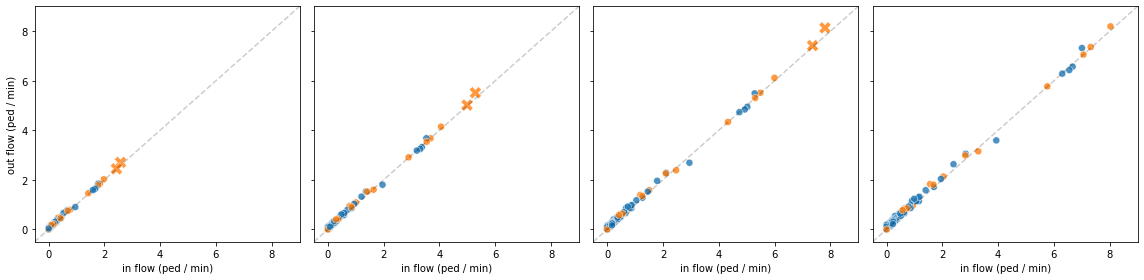
\includegraphics[width=\textwidth]{images/analisi/comparison-base-in-out-flow-ped.png}
        \caption{Modello base}
    \end{subfigure}

    \begin{subfigure}{\textwidth}
        \centering
        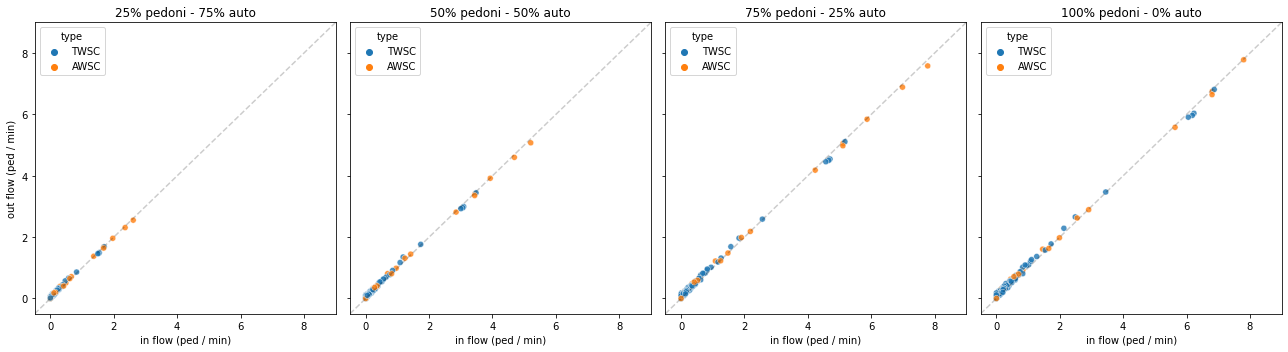
\includegraphics[width=\textwidth]{images/analisi/comparison-new-in-out-flow-ped.png}
        \caption{Modello esteso}
    \end{subfigure}
    \caption{
        Confronto tra il flusso dei pedoni in entrata e in uscita per ogni intersezione al crescere del numero di pedoni.
    }
    \label{fig:analisi-comparison-in-out-flow-ped}
\end{figure}

Osservando il flusso delle auto (Fig. \ref{fig:analisi-comparison-in-out-flow-car})
viene sempre riscontrato un incremento di flusso all'aumentare del numero di auto.

In questo caso però il flusso in entrata e in uscita non sono perfettamente bilanciati e risultano più sparsi rispetto al flusso dei pedoni.
Inoltre in molte intersezioni il flusso in entrata è maggiore del flusso in uscita.

Nel modello esteso il flusso risulta più basso
probabilmente a causa della gestione delle intersezioni che, combinato all'utilizzo dello \textit{shortest path},
provoca un rallentamento al traffico in uscita che, propagandosi in tutta la rete, abbassa il flusso in tutte le intersezioni.

\begin{figure}[ht]
    \centering
    \begin{subfigure}{\textwidth}
        \centering
        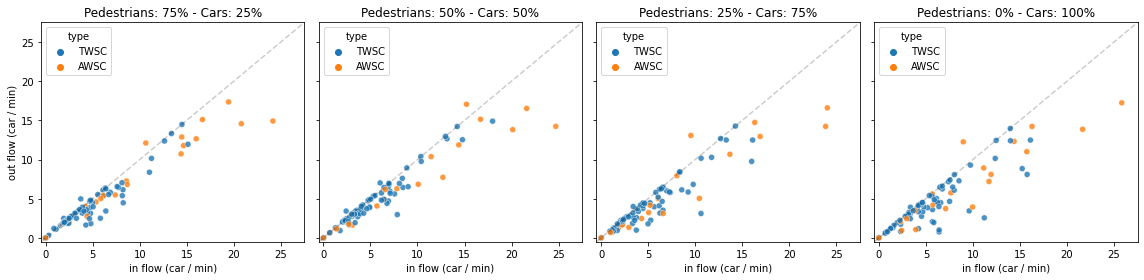
\includegraphics[width=\textwidth]{images/analisi/comparison-base-in-out-flow-car.png}
        \caption{Modello base}
    \end{subfigure}

    \begin{subfigure}{\textwidth}
        \centering
        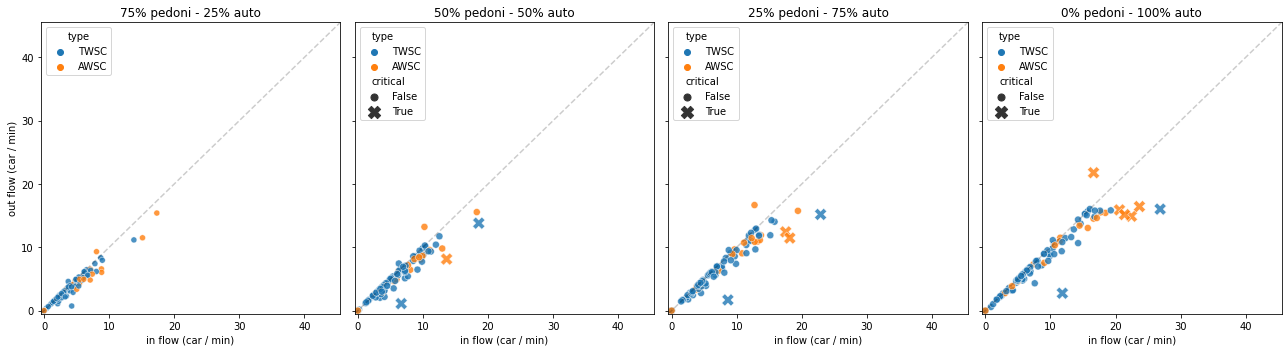
\includegraphics[width=\textwidth]{images/analisi/comparison-new-in-out-flow-car.png}
        \caption{Modello esteso}
    \end{subfigure}
    \caption{
        Confronto tra il flusso delle auto in entrata e in uscita per ogni intersezione al crescere del numero di auto.
    }
    \label{fig:analisi-comparison-in-out-flow-car}
\end{figure}

\pagebreak


\subsubsection*{Tempi di Attesa}

Infine, esclusivamente per il modello esteso, vengono analizzati i tempi di attesa nelle intersezioni per le auto,
ovvero il tempo che passa da quando un'auto arriva all'incrocio a quando ottiene il via libera.
Inoltre i tempi sono distinti tra i due tipi di intersezione: AWSC e TWSC.

Come si può vedere nella tabella \ref{tab:analisi-car-delay}, all'aumentare del numero di auto entrambi i tipi di intersezioni
hanno tempi medi di attesa più lunghi.

Per quanto riguarda le intersezioni TWSC, i tempi di attesa medi e massimi in generale sono più alti rispetto agli AWSC,
per via della presenza degli stop nelle strade secondarie.

\begin{table}[ht]
    \centering
    \begin{tabular}{|c|c|c|c|c|c|}
        \hline
             & 25\% cars & 50\% cars & 75\% cars & 100\% cars & intersection \\ \hline
        mean & 36 s      & 56 s      & 142 s     & 185 s      & AWSC         \\ \hline
        max  & 223 s     & 209 s     & 962 s     & 1363 s     & AWSC         \\ \hline
        mean & 35 s      & 111 s     & 170 s     & 262 s      & TWSC         \\ \hline
        max  & 451 s     & 1136 s    & 1246 s    & 1400 s     & TWSC         \\ \hline
    \end{tabular}
    \caption{Confronto dei tempi di attesa massimi e medi per i due tipi di intersezioni al variare della percentuale di auto considerate.}
    \label{tab:analisi-car-delay}
\end{table}

Nella figura \ref{fig:analisi-comparison-car-delay} vengono riportati i tempi di attesa nella rete al variare del numero di auto.

Al crescere del numero di auto si può notare come la zona in alto vicino al mare composta da una serie di TWSC abbia tempi di attesa più
alti.

Spazialmente si può notare che la maggior parte delle intersezioni con tempi di attesa elevati si trovano vicino al mare.

\begin{figure}[ht]
    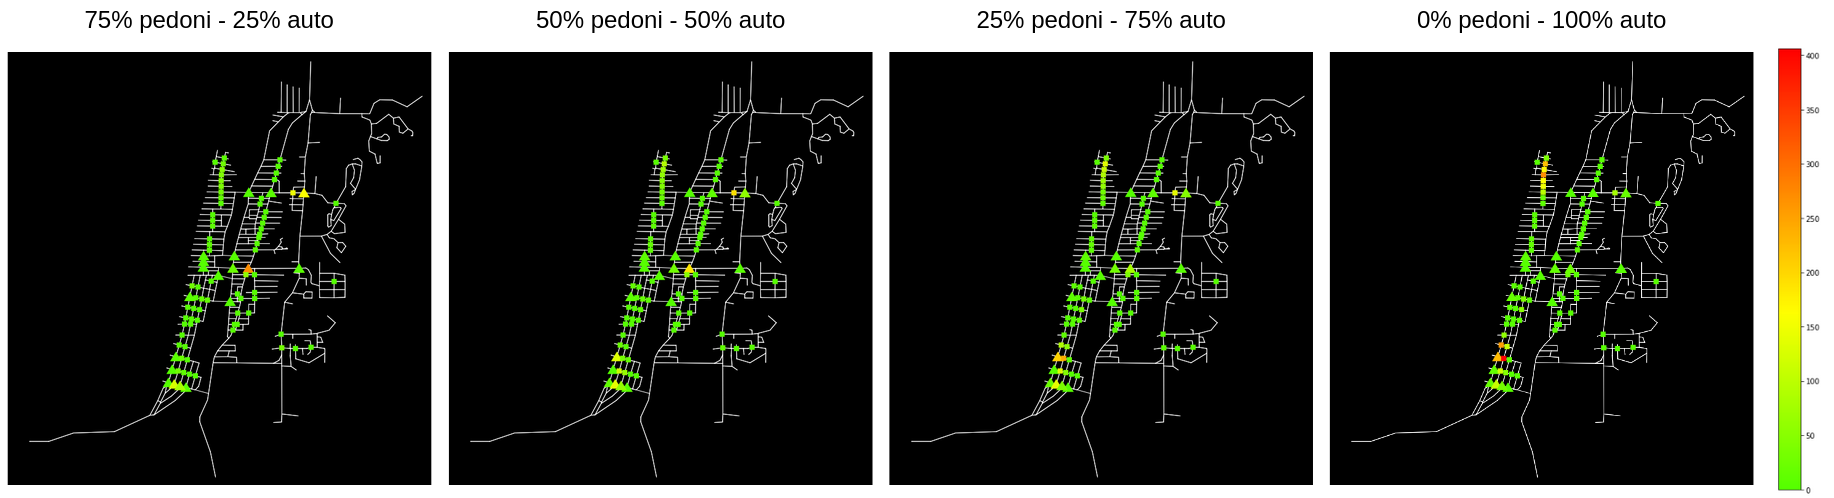
\includegraphics[width=1\textwidth]{images/analisi/comparison-car-delay.png}
    \caption{Tempi di attesa nelle intersezioni al variare del numero di auto, differenziando AWSC (triangoli) e TWSC (cerchi).}
    \label{fig:analisi-comparison-car-delay}
\end{figure}


\subsection{Comparazione con Z. Wang e Jia (2021)}
In questa sezione verranno comparati il modello base e il modello esteso con il modello di \textcite{wang2021novel}, 
il quale rappresenta un modello recente allo stato dell'arte e considera lo stesso scenario di evacuazione di questo lavoro.

\textcite{wang2021novel} hanno effettuato 4000 simulazioni con 5000 agenti e
hanno modellato l'incertezza della percentuale di auto con una variabile $p_c \sim N(\mu_c, \sigma_c)$ troncata in (0, 1), 
dove $\mu_c$ segue una distribuzione uniforme in [0, 1] e $\sigma_c$ = 0.15.
Inoltre sono stati considerati diversi casi che introducono o meno diverse caratteristiche nel modello (Tab. \ref{tab:cases}).

\begin{table}[ht]
    \centering
    \begin{tabular}{|c|c|c|c|}
    \hline
    Cases & Seismic damage & Pedestrian-vehicle interaction & Speed adjustment \\ \hline
    C0 & No  & No  & No  \\ \hline
    C1 & No  & No  & Yes \\ \hline
    C2 & No  & Yes & Yes \\ \hline
    C3 & Yes & No  & Yes \\ \hline
    C4 & Yes & Yes & Yes \\ \hline
    \end{tabular}
    \caption{Casi di simulazione del modello \textcite{wang2021novel}.}
    \label{tab:cases}
\end{table}

Per comparare con il modello di \textcite{wang2021novel} sono state mediate le prove effettuate al variare del numero
di auto e di pedoni con un totale di 4502 agenti (Fig. \ref{fig:analisi-comparison-wang2}).
Nella comparazione verranno presi in considerazione esclusivamente i casi C0, C1 e C2, ovvero quelli
che non gestiscono i danni sismici.

\begin{figure}[ht]
    \centering
    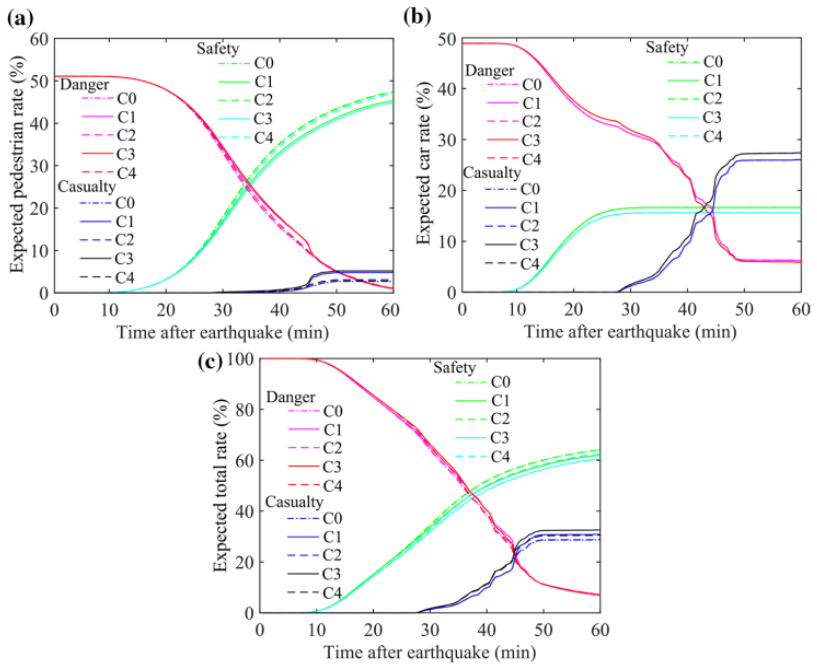
\includegraphics[width=\textwidth]{images/analisi/WANG_comparison1.png}
    \caption{Confronto della percentuali di evacuati e di vittime per auto, pedoni e totale per il modello di \textcite{wang2021novel}.}
    \label{fig:analisi-comparison-wang1}
\end{figure}

\begin{figure}[ht]
    \centering
    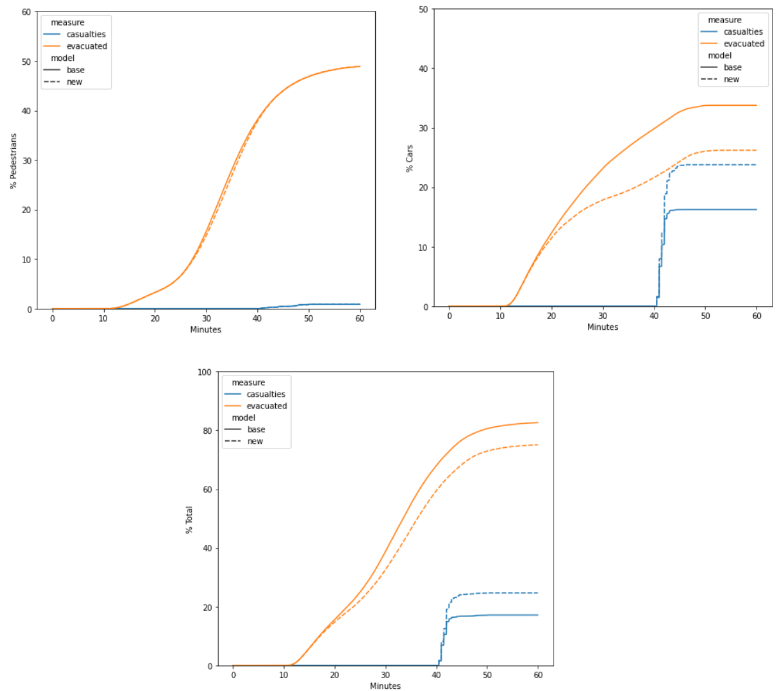
\includegraphics[width=\textwidth]{images/analisi/WANG_comparison2.png}
    \caption{Confronto della percentuali di evacuati e di vittime per auto, pedoni e totale per modello base ed esteso.}
    \label{fig:analisi-comparison-wang2}
\end{figure}

Come si nota nella figura \ref{fig:analisi-comparison-wang1} in entrambi i modelli i primi agenti
iniziano a evacuare intorno ai 10 minuti. Nel caso di \textcite{wang2021novel} le auto iniziano
poco prima dei 10 minuti per via dei parametri della distribuzione di Rayleigh.

Nel modello di \textcite{wang2021novel} le prime vittime si verificano a circa 28 minuti ovvero quando lo tsunami inizia ad arrivare alla costa, 
mentre nel modello esteso e nel modello base dopo 40 minuti, ovvero quando lo tsunami ha già coperto l'area vicino alla costa. 
Dopo 50 minuti lo tsunami ha raggiunto la massima distanza e infatti in tutti i modelli il numero di vittime rimane costante.

Osservando solo i pedoni si può notare come il caso C2 sia lo scenario più simile ai risultati 
ottenuti dal modello base ed esteso per vittime ed evacuati, con valori leggermente inferiori di evacuati e maggiori di vittime.
Sono presenti comunque delle differenze dovute ad diversi tempi di partenza degli agenti, alla larghezza della strada considerata ed un numero diverso di agenti.
Infatti nel modello di \textcite{wang2021novel} l'andamento risulta leggermente più veloce tra i 20 e i 30 minuti
e leggermente più lento dopo i 35 minuti.
Inoltre nel modello di \textcite{wang2021novel} c'è una differenza più significativa
nell'effettuare una variazione della velocità dei pedoni casi C0 e C1, 
rispetto alla differenza tra il modello base ed esteso.

In tutti i modelli le auto presentano differenze più marcate sia per le vittime che per gli evacuati. 
Nel modello di \textcite{wang2021novel} gli evacuati hanno una curva crescente fino a circa 30 minuti dopo i quali si appiattisce e raggiunge un valore di circa 17\%, 
mentre nel modello base e nel modello esteso la curva continua a crescere fino a 50 minuti e raggiunge un valore di 34\% nel modello base e di 26\% nel modello esteso.
Per quanto riguarda le vittime nel modello di \textcite{wang2021novel} l'andamento cresce lentamente tra 28 e circa 50 minuti raggiungendo un valore di 26\%, mentre nel
modello base e nel modello esteso la maggior parte delle vittime è concetrata vicino a 40 minuti raggiungendo un valore di di 16\% nel modello base e di 24\% nel modello esteso.

Nel caso totale sono presenti andamenti simili a quelli già descritti nei grafici per i pedoni e per le auto. 
Il modello base e il modello esteso prevedono un numero maggiore di evacuati e un numero minore di vittime rispetto al modello di \textcite{wang2021novel}.
In particolare si può notare un massimo di evacuati dell'82\% per il modello base e un massimo di vittime del 25\% per il modello esteso,
mentre per i casi C0, C1 e C2 sono previsti un numero massimo di evacuati poco sopra il 60\% e un numero massimo di vittime di circa 30\%.

\newpage
